\begin{figure}[htbp]
    \captionsetup[subfigure]{justification=centering}
    \centering
    \begin{subfigure}[b]{0.3\textwidth}
        \centering
        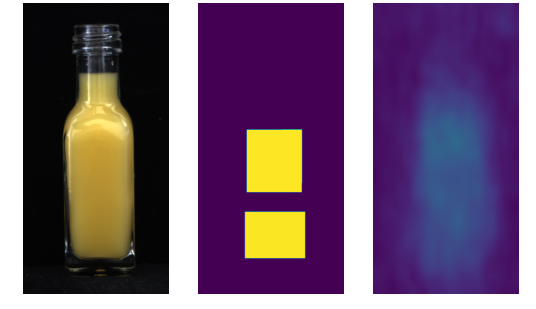
\includegraphics[width=\textwidth]{figures/locosimplenetresults/JB/image_prediction_105.png}
        %\caption*{Logical Anomalies}

    \end{subfigure}
    \begin{subfigure}[b]{0.3\textwidth}
        \centering
        %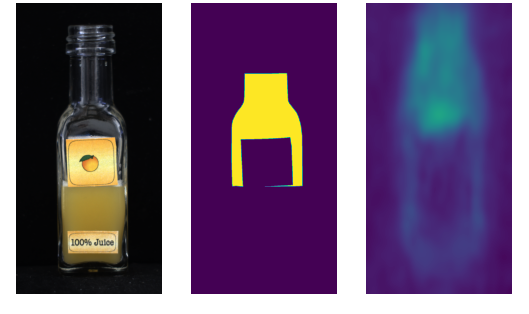
\includegraphics[width=\textwidth]{figures/locosimplenetresults/JB/image_prediction_188.png}

    \end{subfigure}
    \begin{subfigure}[b]{0.3\textwidth}
        \centering
        %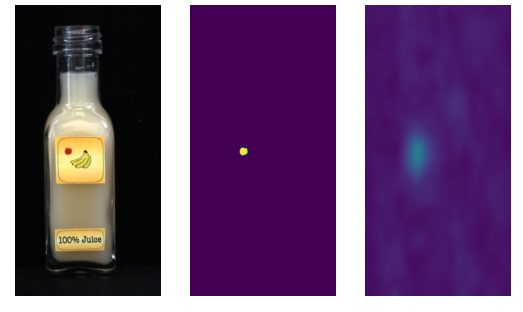
\includegraphics[width=\textwidth]{figures/locosimplenetresults/JB/image_prediction_258.png}

    \end{subfigure}
    \begin{subfigure}[b]{0.3\textwidth}
        \centering
        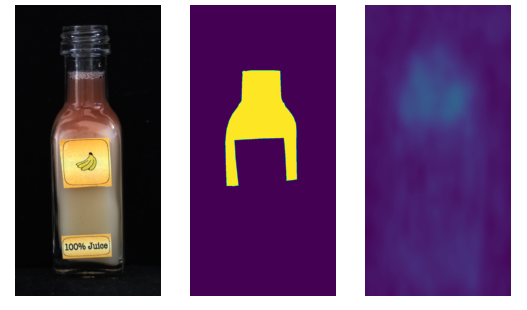
\includegraphics[width=\textwidth]{figures/locosimplenetresults/JB/image_prediction_286.png}
                %\caption*{Structural Anomalies}

    \end{subfigure}
    \begin{subfigure}[b]{0.3\textwidth}
        \centering
        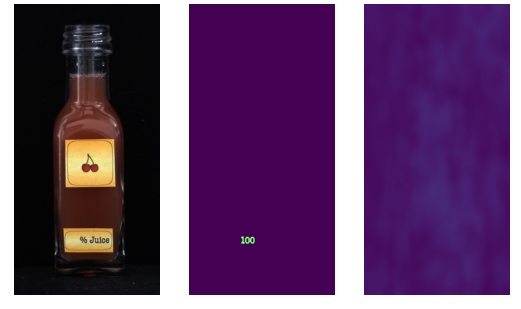
\includegraphics[width=\textwidth]{figures/locosimplenetresults/JB/image_prediction_297.png}

    \end{subfigure}
    \begin{subfigure}[b]{0.3\textwidth}
        \centering
        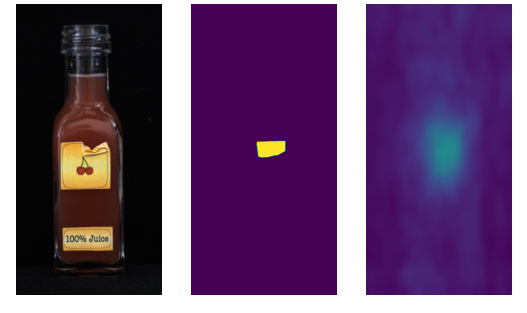
\includegraphics[width=\textwidth]{figures/locosimplenetresults/JB/image_prediction_300.png}

    \end{subfigure}
    \caption{Representative segmentation results from SimpleNet \cite{liu2023simplenet} on the juice bottle class of the MVTecAD LOCO \cite{LOCODentsAndScratchesBergmann2022} dataset.}
    \label{fig:SNJB}
\end{figure}